\section{Servizi di rete}
\subsection{DNS}
Dato che ricordarsi a memoria gli indirizzi ip di un dispositivo è faticoso e poco funzionale, Cisco Packet Tracert offre anche la possibilità di attivare il servizio DNS. L’acronimo DNS sta per Domain Name System, cioè permette di tradurre gli indirizzi ip in nomi o frasi che possiamo decidere noi. In questo modo, non dobbiamo più ricordarci una serie di numeri, piuttosto una stringa, come può essere “google.com” o “youtube.com”, generalmente più facili da ricordare.

Per poter abilitare questo servizio, bisogna nuovamente avere a disposizione un server all’interno della propria rete. Da qui, dobbiamo seguire una serie di passaggi specifici:

\begin{enumerate}
    \item Aprire la schermata “servizi” e selezionare la scheda “DNS”.
    \item Assicurarsi che la spunta relativa sia settata su on.
    \item Selezionando il campo “name” è possibile scegliere il nome del sito. Per esempio, “www.sito.com”.
    \item Sullo spazio “address”, bisogna inserire l’indirizzo ip della macchina che contiene il sito internet.
    \item Premere su add per salvare queste impostazioni.
    \item Il procedimento è andato a buon fine. Per verificare, si può provare a connettersi al server tramite DNS con un pc. Tale pc avrà bisogno dell’indirizzo DNS inserito nelle impostazioni attraverso Desktop, configurazione IP.
\end{enumerate}

\begin{figure}[htbp]
    \centering
    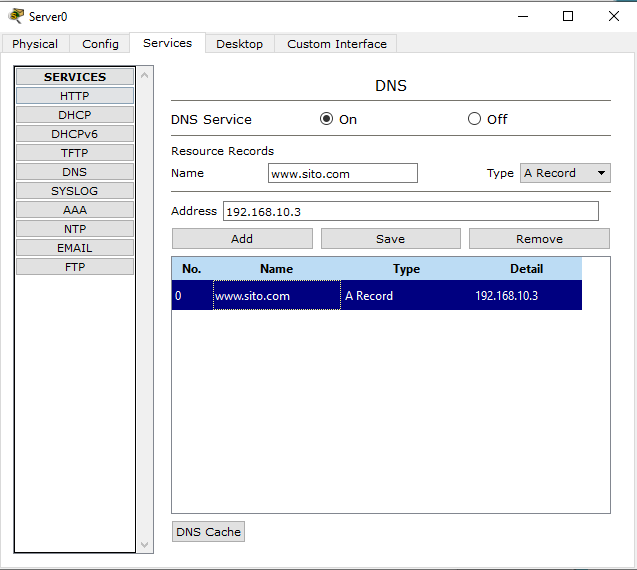
\includegraphics[width=0.5\textwidth]{images/06.servizi-rete/dns/01.conf-server.png}
    \caption{Esempio di schermata del servizio DNS.}
    \label{fig:dns-conf-server}
\end{figure}

\begin{figure}[htbp]
    \centering
    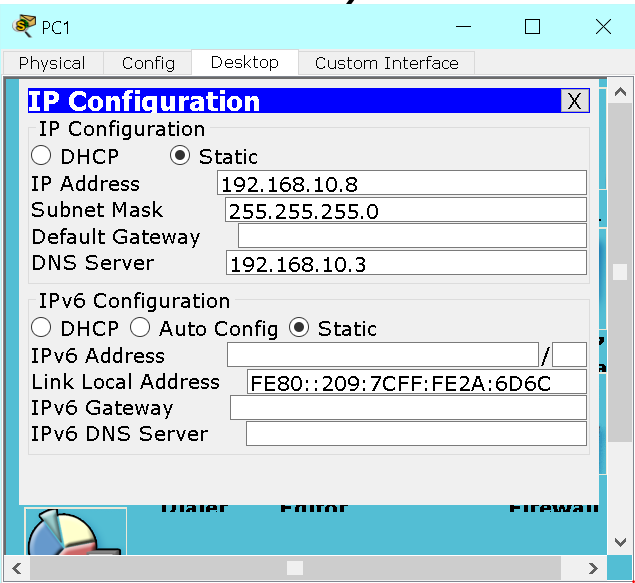
\includegraphics[width=0.5\textwidth]{images/06.servizi-rete/dns/02.conf-pc.png}
    \caption{Configurazione indirizzo server DNS nel pc.}
    \label{fig:dns-conf-pc}
\end{figure}

\begin{figure}[htbp]
    \centering
    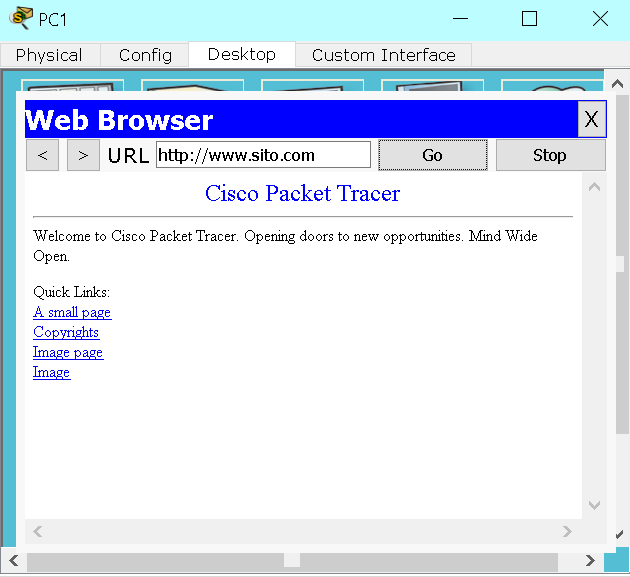
\includegraphics[width=0.5\textwidth]{images/06.servizi-rete/dns/03.test.png}
    \caption{Prova funzionamento del DNS}
    \label{fig:dns-test}
\end{figure}

\subsection{DHCP}
\subsubsection{Server router}
\subsubsection{Server specializzato}
\subsection{EMAIL}
Un ulteriore servizio offerto da Cisco Packet Tracert è il servizio Email. Tale servizio permette di avere la funzionalità della posta elettronica in una singola rete o più reti. Così gli utenti possono scambiarsi messaggi virtuali e avere profili con username e password.

Per attivare questo servizio, bisogna seguire dei determinati passaggi:

\begin{enumerate}
    \item Aprire la schermata “servizi” e selezionare la scheda “Email”.
    \item Assicurarsi che le spunte relative al SMTP e POP3 siano settata su on.
    \item Su “domain name”, inserire il nome del dominio del servizio email. Un esempio può essere “dominio.com”.
    \item Sotto, su user bisogna inserire l’username di un determinato profilo, con l’aggiunta della password. Una volta scelti entrambi, cliccando sul tasto “+” è possibile aggiungere quel determinato utente.
    \item Il servizio è ora attivo e funzionante. Per usufruirne, bisogna selezionare un pc, recarsi nella tab “desktop” e selezionare “Email”. Nella prima schermata di configurazione, bisogna inserire i dati che sono stati aggiunti nella tab Email del server. Su Email address bisogna inserire username + @ + dominio (es: “utente1@dominio.com”) . Sui due campi Incoming e Outgoing Mail Server bisogna inserire l’ip della macchina che hosta il servizio. Una volta configurato l’account, è possibile quindi utilizzare il servizio.
    \item Cliccando su Compose è possibile inviare una mail ad un determinato indirizzo di posta. Cliccando su Reply è possibile rispondere ad una mail che si è ricevuta. Cliccando su Receive è possibile aggiornare le email ricevute. Cliccando su delete è possibile cancellare le email ricevute.
\end{enumerate}

\begin{figure}[htbp]
    \centering
    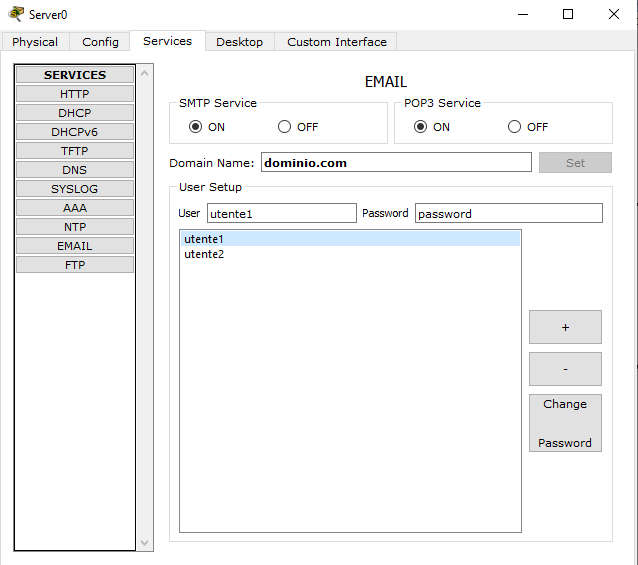
\includegraphics[width=0.5\textwidth]{images/06.servizi-rete/email/01.conf-server.png}
    \caption{Esempio di schermata del servizio Email.}
    \label{fig:email-conf-server}
\end{figure}

\begin{figure}[htbp]
    \centering
    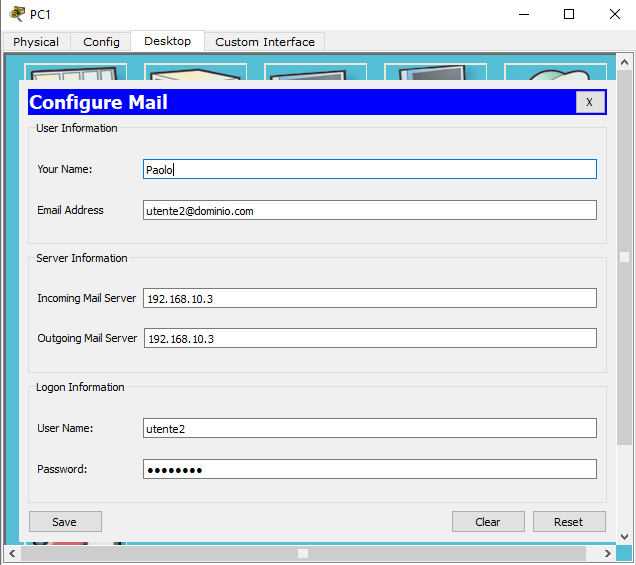
\includegraphics[width=0.5\textwidth]{images/06.servizi-rete/email/02.test.png}
    \caption{Esempio di configurazione dell’utente.}
    \label{fig:email-conf-client}
\end{figure}

\subsection{HTTP}
Cisco Packet Tracert offre, in aggiunta, il servizio HTTP, così da permettere a più utenti di una singola rete o di più reti per accedere ad un sito internet completamente configurabile. L’HTTP (HyperText Transfer Protocol) di per sé è un insieme di regole che un server deve seguire quando si tratta della trasmissione di file attraverso il World Wide Web. La base del funzionamento di tale protocollo è che ogni file o pagina è collegato a altri file attraverso una serie di collegamenti. Esiste una versione più sicura del HTTP chiamato HTTPS che, aggiungendo la crittografia dei dati sensibili, permette una maggiore sicurezza durante l’invio dei pacchetti.

Per abilitare il servizio HTTP su Cisco Packet Tracert, bisogna avere a disposizione un server all’interno della propria rete, così che sia collegato ad altre apparecchiature. Per poter abilitare il tutto, quindi, bisogna seguire dei passaggi specifici:

\begin{enumerate}
    \item Aprire la schermata “servizi” del server.
    \item Selezionare la scheda HTTP.
    \item Assicurarsi che le due spunte relative all’HTTP e all’HTTPS siano impostate su “on”.
    \item I due servizi sono quindi attivi. Adesso è possibile aggiungere, modificare o eliminare pagine html, che saranno quelle che comporranno il sito gestito dal server.
    \item Per potersi connettere a questo sito, bisogna avere a disposizione di un pc che sia connesso alla rete del server. Dopo aver aperto la schermata “Web Browser” dalla scheda desktop del pc, è possibile inserire l’indirizzo ip del server, così da connettersi al suo sito. Di default, la prima pagina è la “index.html”.
\end{enumerate}

\begin{figure}[htbp]
    \centering
    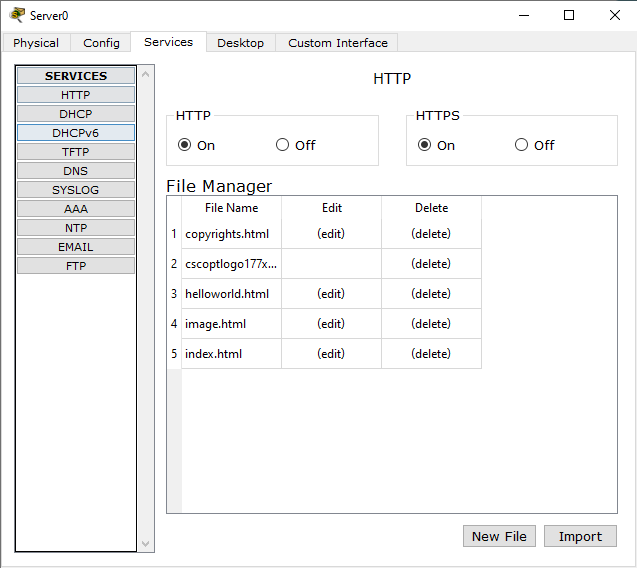
\includegraphics[width=0.5\textwidth]{images/06.servizi-rete/http/01.conf-server.png}
    \caption{Esempio di schermata HTTP di un server. Da qui è possibile cancellare, modificare o aggiungere una nuova pagina html.}
    \label{fig:http-conf}
\end{figure}

\begin{figure}[htbp]
    \centering
    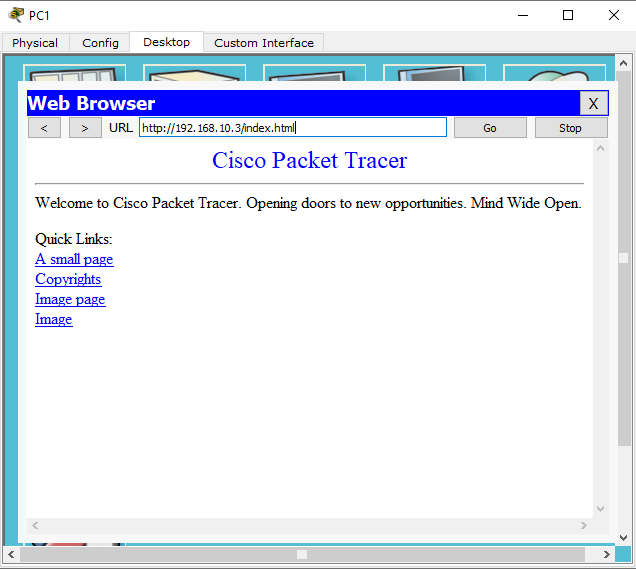
\includegraphics[width=0.5\textwidth]{images/06.servizi-rete/http/02.conf-client.png}
    \caption{Esempio di collegamento alla pagina index di un sito. Nell’URL va inserito l’indirizzo del server + / + nome della pagina.}
    \label{fig:http-test}
\end{figure}